%%%%%%%%%%%%%%%%%%%%%%%%%%%%%%%%%%%%%%%%%%%%%%%%%%%%%%%%%%%%
% 1.14 UNIVERSAL ALGEBRA
% The Composition of Advanced Mathematics
%%%%%%%%%%%%%%%%%%%%%%%%%%%%%%%%%%%%%%%%%%%%%%%%%%%%%%%%%%%%

\section{Universal Algebra}
\label{sec:universal-algebra}

\prerequisite{
Abstract algebra from \cref{sec:abstract-algebra}, group theory from
\cref{sec:group-theory}, ring theory from \cref{sec:ring-theory}, and basic
set-theoretic functions and relations from \cref{sec:functions,sec:relations}.
}

\learningobjectives{
By the end of this section, the reader should be able to:
\begin{itemize}
    \item explain the purpose of universal algebra;
    \item define finitary operations and algebraic signatures;
    \item describe an algebra of a specified type;
    \item recognize groups, rings, lattices, and related structures as algebras;
    \item define subalgebras, generated subalgebras, and homomorphisms;
    \item define congruence relations and quotient algebras;
    \item explain kernels of homomorphisms as congruences;
    \item state and apply the First Isomorphism Theorem for universal algebras;
    \item distinguish identities from arbitrary logical statements;
    \item define varieties and understand Birkhoff's HSP theorem;
    \item construct and interpret term algebras and free algebras;
    \item explain direct products of algebras;
    \item understand congruence lattices at an introductory level;
    \item recognize the relationship between universal algebra, logic,
    lattice theory, and category theory.
\end{itemize}
}

%%%%%%%%%%%%%%%%%%%%%%%%%%%%%%%%%%%%%%%%%%%%%%%%%%%%%%%%%%%%
\subsection{What Is Universal Algebra?}
\label{subsec:what-is-universal-algebra}
%%%%%%%%%%%%%%%%%%%%%%%%%%%%%%%%%%%%%%%%%%%%%%%%%%%%%%%%%%%%

Group theory studies groups, ring theory studies rings, and lattice theory
studies lattices. These structures look different, but they share many
structural features.

Each consists of:

\begin{itemize}
    \item an underlying set;
    \item one or more operations;
    \item identities satisfied by those operations;
    \item substructures;
    \item homomorphisms;
    \item congruence relations;
    \item quotient structures;
    \item products.
\end{itemize}

Universal algebra studies these common patterns simultaneously.

\begin{conceptbox}
\textbf{Universal algebra} studies algebraic structures abstractly through
their operations and identities rather than concentrating on one particular
kind of algebraic object.
\end{conceptbox}

The central idea is to replace statements such as

``let \(G\) be a group''

with the more general statement

``let \(A\) be an algebra having operations of specified arities.''

%%%%%%%%%%%%%%%%%%%%%%%%%%%%%%%%%%%%%%%%%%%%%%%%%%%%%%%%%%%%
\subsection{The Universal-Algebra Viewpoint}
\label{subsec:universal-algebra-viewpoint}
%%%%%%%%%%%%%%%%%%%%%%%%%%%%%%%%%%%%%%%%%%%%%%%%%%%%%%%%%%%%

The progression can be visualized as

\begin{center}
\begin{tikzpicture}[
    node distance=8mm and 12mm,
    box/.style={draw,rounded corners,align=center,inner sep=5pt},
    >=stealth
]
\node[box] (groups) {Groups};
\node[box,right=of groups] (rings) {Rings};
\node[box,right=of rings] (lattices) {Lattices};
\node[box,right=of lattices] (others) {Other\\algebras};

\node[box,below=18mm of $(rings)!0.5!(lattices)$] (univ)
{Universal Algebra\\operations + identities};

\draw[->] (groups)--(univ);
\draw[->] (rings)--(univ);
\draw[->] (lattices)--(univ);
\draw[->] (others)--(univ);
\end{tikzpicture}
\end{center}

Universal algebra does not replace the individual theories. Instead, it
extracts results that depend only on general algebraic structure.

%%%%%%%%%%%%%%%%%%%%%%%%%%%%%%%%%%%%%%%%%%%%%%%%%%%%%%%%%%%%
\subsection{Operations}
\label{subsec:universal-operations}
%%%%%%%%%%%%%%%%%%%%%%%%%%%%%%%%%%%%%%%%%%%%%%%%%%%%%%%%%%%%

The most basic ingredient is an operation.

\begin{definitionbox}{\(n\)-ary Operation}
Let \(A\) be a set and let \(n\in\N\). An \emph{\(n\)-ary operation} on
\(A\) is a function
\[ f:A^n\to A. \]
\end{definitionbox}

The word \emph{arity} refers to the number of inputs accepted by an
operation.

Thus an \(n\)-ary operation has arity \(n\).

%%%%%%%%%%%%%%%%%%%%%%%%%%%%%%%%%%%%%%%%%%%%%%%%%%%%%%%%%%%%
\subsection{Nullary, Unary, and Binary Operations}
\label{subsec:operation-arities}
%%%%%%%%%%%%%%%%%%%%%%%%%%%%%%%%%%%%%%%%%%%%%%%%%%%%%%%%%%%%

Several arities occur frequently.

A \emph{nullary operation} has no input and represents a distinguished
constant.

A \emph{unary operation} has one input:

\[ f:A\to A. \]

A \emph{binary operation} has two inputs:

\[ f:A^2\to A. \]

A ternary operation has three inputs:

\[ f:A^3\to A. \]

\begin{center}
\begin{tabularx}{0.88\textwidth}{@{}lllX@{}}
\toprule
\textbf{Arity} & \textbf{Name} & \textbf{Form} & \textbf{Example}\\
\midrule
\(0\) & nullary & constant & identity element \(e\)\\
\(1\) & unary & \(A\to A\) & inverse \(x\mapsto x^{-1}\)\\
\(2\) & binary & \(A^2\to A\) & addition or multiplication\\
\(3\) & ternary & \(A^3\to A\) & a three-input operation\\
\(n\) & \(n\)-ary & \(A^n\to A\) & general operation\\
\bottomrule
\end{tabularx}
\end{center}

%%%%%%%%%%%%%%%%%%%%%%%%%%%%%%%%%%%%%%%%%%%%%%%%%%%%%%%%%%%%
\subsection{Finitary Operations}
\label{subsec:finitary-operations}
%%%%%%%%%%%%%%%%%%%%%%%%%%%%%%%%%%%%%%%%%%%%%%%%%%%%%%%%%%%%

An operation is called \emph{finitary} when it accepts finitely many inputs.

Classical universal algebra primarily studies structures equipped with
finitary operations.

This includes essentially all familiar elementary algebraic structures such
as groups, rings, modules, and lattices.

%%%%%%%%%%%%%%%%%%%%%%%%%%%%%%%%%%%%%%%%%%%%%%%%%%%%%%%%%%%%
\subsection{Signatures}
\label{subsec:signatures}
%%%%%%%%%%%%%%%%%%%%%%%%%%%%%%%%%%%%%%%%%%%%%%%%%%%%%%%%%%%%

To describe a type of algebra, one must specify which operation symbols are
available and how many inputs each accepts.

\begin{definitionbox}{Signature}
A \emph{signature}, also called a \emph{type} or \emph{similarity type}, is
a collection of operation symbols together with an assigned arity for each
symbol.
\end{definitionbox}

A signature is often denoted by

\[ \Sigma. \]

The symbol \(\Sigma\) is the uppercase Greek letter \emph{sigma},
pronounced ``SIG-muh.''

Here it represents the collection of operation symbols defining an
algebraic language.

%%%%%%%%%%%%%%%%%%%%%%%%%%%%%%%%%%%%%%%%%%%%%%%%%%%%%%%%%%%%
\subsection{Examples of Signatures}
\label{subsec:signature-examples}
%%%%%%%%%%%%%%%%%%%%%%%%%%%%%%%%%%%%%%%%%%%%%%%%%%%%%%%%%%%%

A group may be represented by the signature

\[ \Sigma_{\mathrm{Grp}}=\{\cdot,{}^{-1},e\}, \]

where

\begin{itemize}
    \item \(\cdot\) is binary;
    \item \(^{-1}\) is unary;
    \item \(e\) is nullary.
\end{itemize}

A ring may use

\[ \Sigma_{\mathrm{Ring}}=\{+,-,\cdot,0,1\}, \]

where \(+\) and \(\cdot\) are binary, negation is unary, and \(0,1\) are
nullary.

A lattice may use

\[ \Sigma_{\mathrm{Lat}}=\{\wedge,\vee\}. \]

The symbols \(\wedge\) and \(\vee\) are read ``meet'' and ``join,''
respectively, in lattice theory.

%%%%%%%%%%%%%%%%%%%%%%%%%%%%%%%%%%%%%%%%%%%%%%%%%%%%%%%%%%%%
\subsection{Algebras of a Signature}
\label{subsec:algebras-signature}
%%%%%%%%%%%%%%%%%%%%%%%%%%%%%%%%%%%%%%%%%%%%%%%%%%%%%%%%%%%%

\begin{definitionbox}{Algebra}
Let \(\Sigma\) be a signature. A \emph{\(\Sigma\)-algebra} consists of a
nonempty set \(A\) together with an interpretation
\[ f^A:A^n\to A \]
for every \(n\)-ary operation symbol \(f\in\Sigma\).
\end{definitionbox}

The superscript in

\[ f^A \]

is read ``\(f\) interpreted in \(A\).''

It distinguishes an abstract operation symbol \(f\) from the concrete
operation it represents on the set \(A\).

An algebra is often written

\[ \mathbf{A}=(A,(f^A)_{f\in\Sigma}). \]

The bold symbol \(\mathbf{A}\) refers to the entire algebraic structure,
while \(A\) refers to its underlying set.

%%%%%%%%%%%%%%%%%%%%%%%%%%%%%%%%%%%%%%%%%%%%%%%%%%%%%%%%%%%%
\subsection{Structure of an Algebra}
\label{subsec:structure-of-algebra}
%%%%%%%%%%%%%%%%%%%%%%%%%%%%%%%%%%%%%%%%%%%%%%%%%%%%%%%%%%%%

\begin{center}
\begin{tikzpicture}[
    node distance=10mm,
    box/.style={draw,rounded corners,align=center,inner sep=6pt},
    >=stealth
]
\node[box] (alg) {\(\Sigma\)-algebra \(\mathbf A\)};
\node[box,below left=of alg] (set) {Underlying set\\\(A\)};
\node[box,below right=of alg] (ops) {Operations\\\(f^A\)};
\node[box,below=of ops] (arity) {Specified arities};

\draw[->] (alg)--(set);
\draw[->] (alg)--(ops);
\draw[->] (ops)--(arity);
\end{tikzpicture}
\end{center}

The signature determines the \emph{shape} of the structure.

The algebra determines how those operations actually behave.

%%%%%%%%%%%%%%%%%%%%%%%%%%%%%%%%%%%%%%%%%%%%%%%%%%%%%%%%%%%%
\subsection{Groups as Universal Algebras}
\label{subsec:groups-universal-algebras}
%%%%%%%%%%%%%%%%%%%%%%%%%%%%%%%%%%%%%%%%%%%%%%%%%%%%%%%%%%%%

A group

\[ (G,\cdot,{}^{-1},e) \]

is an algebra with:

\begin{itemize}
    \item one binary operation;
    \item one unary operation;
    \item one distinguished constant.
\end{itemize}

The group axioms are identities involving these operations.

For example, associativity is

\[ (xy)z=x(yz). \]

The identity laws are

\[ ex=x,\qquad xe=x. \]

The inverse laws are

\[ xx^{-1}=e,\qquad x^{-1}x=e. \]

Thus group theory fits naturally inside universal algebra.

%%%%%%%%%%%%%%%%%%%%%%%%%%%%%%%%%%%%%%%%%%%%%%%%%%%%%%%%%%%%
\subsection{Rings as Universal Algebras}
\label{subsec:rings-universal-algebras}
%%%%%%%%%%%%%%%%%%%%%%%%%%%%%%%%%%%%%%%%%%%%%%%%%%%%%%%%%%%%

A unital ring can be viewed as

\[ (R,+,-,\cdot,0,1). \]

Its identities include associativity of addition and multiplication,
additive commutativity, additive inverses, distributivity, and identity
laws.

For example,

\[ x(y+z)=xy+xz. \]

From the universal-algebra viewpoint, the important point is that all of
these laws are equations between terms.

%%%%%%%%%%%%%%%%%%%%%%%%%%%%%%%%%%%%%%%%%%%%%%%%%%%%%%%%%%%%
\subsection{Terms}
\label{subsec:universal-terms}
%%%%%%%%%%%%%%%%%%%%%%%%%%%%%%%%%%%%%%%%%%%%%%%%%%%%%%%%%%%%

Terms are formal expressions built from variables and operation symbols.

\begin{definitionbox}{Term}
A \emph{term} in a signature \(\Sigma\) is constructed recursively from
variables and the operation symbols in \(\Sigma\).
\end{definitionbox}

For a group signature, examples include

\[ x,\qquad e,\qquad x^{-1},\qquad xy,\qquad x(y^{-1}z). \]

For a ring signature, examples include

\[ x+y,\qquad xy,\qquad x(y+z),\qquad x^2+xy+1. \]

Terms are syntactic objects until interpreted in a particular algebra.

%%%%%%%%%%%%%%%%%%%%%%%%%%%%%%%%%%%%%%%%%%%%%%%%%%%%%%%%%%%%
\subsection{Term Evaluation}
\label{subsec:term-evaluation}
%%%%%%%%%%%%%%%%%%%%%%%%%%%%%%%%%%%%%%%%%%%%%%%%%%%%%%%%%%%%

Suppose

\[ t(x_1,\ldots,x_n) \]

is a term and \(\mathbf A\) is a \(\Sigma\)-algebra.

The term determines a function

\[ t^{\mathbf A}:A^n\to A. \]

This is called the \emph{term operation} induced by \(t\).

For example, in a ring,

\[ t(x,y)=x^2+xy+1 \]

induces

\[ t^R(a,b)=a^2+ab+1. \]

%%%%%%%%%%%%%%%%%%%%%%%%%%%%%%%%%%%%%%%%%%%%%%%%%%%%%%%%%%%%
\subsection{Identities}
\label{subsec:universal-identities}
%%%%%%%%%%%%%%%%%%%%%%%%%%%%%%%%%%%%%%%%%%%%%%%%%%%%%%%%%%%%

\begin{definitionbox}{Identity}
An \emph{identity} is a formal equation
\[ s(x_1,\ldots,x_n)\approx t(x_1,\ldots,x_n) \]
between two terms of the same signature.
\end{definitionbox}

The symbol

\[ \approx \]

is read here as ``is identically equal to.''

It emphasizes that the equation is intended as a universal algebraic law,
rather than an equation to solve for particular variables.

An algebra satisfies the identity when

\[ s^{\mathbf A}(a_1,\ldots,a_n)
=t^{\mathbf A}(a_1,\ldots,a_n) \]

for every choice of elements \(a_1,\ldots,a_n\in A\).

%%%%%%%%%%%%%%%%%%%%%%%%%%%%%%%%%%%%%%%%%%%%%%%%%%%%%%%%%%%%
\subsection{Examples of Identities}
\label{subsec:identity-examples}
%%%%%%%%%%%%%%%%%%%%%%%%%%%%%%%%%%%%%%%%%%%%%%%%%%%%%%%%%%%%

Associativity is expressed by

\[ (xy)z\approx x(yz). \]

Commutativity is

\[ xy\approx yx. \]

Idempotence is

\[ x\cdot x\approx x. \]

A lattice satisfies identities such as

\[ x\wedge x\approx x,\qquad x\vee x\approx x. \]

Distributivity of multiplication over addition in rings is

\[ x(y+z)\approx xy+xz. \]

%%%%%%%%%%%%%%%%%%%%%%%%%%%%%%%%%%%%%%%%%%%%%%%%%%%%%%%%%%%%
\subsection{Equational Classes}
\label{subsec:equational-classes}
%%%%%%%%%%%%%%%%%%%%%%%%%%%%%%%%%%%%%%%%%%%%%%%%%%%%%%%%%%%%

A collection of identities can be used to define an entire class of
algebras.

For example, the associative identity

\[ (xy)z\approx x(yz) \]

defines semigroups among algebras having one binary operation.

Adding an identity constant \(e\) satisfying

\[ ex\approx x,\qquad xe\approx x \]

produces monoids.

Adding an inverse operation and inverse identities produces groups.

\begin{center}
\begin{tikzpicture}[
    node distance=8mm,
    box/.style={draw,rounded corners,align=center,inner sep=5pt},
    >=stealth
]
\node[box] (bin) {Binary algebras};
\node[box,below=of bin] (semi) {Semigroups\\associativity};
\node[box,below=of semi] (mon) {Monoids\\identity};
\node[box,below=of mon] (grp) {Groups\\inverses};

\draw[->] (bin)--(semi);
\draw[->] (semi)--(mon);
\draw[->] (mon)--(grp);
\end{tikzpicture}
\end{center}

%%%%%%%%%%%%%%%%%%%%%%%%%%%%%%%%%%%%%%%%%%%%%%%%%%%%%%%%%%%%
\subsection{Subalgebras}
\label{subsec:universal-subalgebras}
%%%%%%%%%%%%%%%%%%%%%%%%%%%%%%%%%%%%%%%%%%%%%%%%%%%%%%%%%%%%

The familiar idea of a subgroup or subring generalizes directly.

\begin{definitionbox}{Subalgebra}
Let \(\mathbf A\) be a \(\Sigma\)-algebra. A subset \(B\subseteq A\) is the
underlying set of a \emph{subalgebra} \(\mathbf B\) if \(B\) is closed under
every fundamental operation of \(\mathbf A\).
\end{definitionbox}

For every \(n\)-ary operation \(f\), closure means

\[ b_1,\ldots,b_n\in B
\quad\Longrightarrow\quad
f^A(b_1,\ldots,b_n)\in B. \]

Nullary operations require all distinguished constants to belong to \(B\).

%%%%%%%%%%%%%%%%%%%%%%%%%%%%%%%%%%%%%%%%%%%%%%%%%%%%%%%%%%%%
\subsection{Generated Subalgebras}
\label{subsec:generated-subalgebras}
%%%%%%%%%%%%%%%%%%%%%%%%%%%%%%%%%%%%%%%%%%%%%%%%%%%%%%%%%%%%

Given

\[ X\subseteq A, \]

one may ask for the smallest subalgebra containing \(X\).

\begin{definitionbox}{Generated Subalgebra}
The \emph{subalgebra generated by \(X\)}, denoted
\[ \langle X\rangle, \]
is the intersection of all subalgebras of \(\mathbf A\) containing \(X\).
\end{definitionbox}

The notation

\[ \langle X\rangle \]

is read ``the subalgebra generated by \(X\).''

Operationally, it consists of elements obtained by repeatedly applying the
fundamental operations to elements of \(X\) and to any distinguished
constants.

%%%%%%%%%%%%%%%%%%%%%%%%%%%%%%%%%%%%%%%%%%%%%%%%%%%%%%%%%%%%
\subsection{Generation as Closure}
\label{subsec:generation-closure}
%%%%%%%%%%%%%%%%%%%%%%%%%%%%%%%%%%%%%%%%%%%%%%%%%%%%%%%%%%%%

The process can be pictured as

\begin{center}
\begin{tikzpicture}[
    node distance=11mm,
    box/.style={draw,rounded corners,align=center,inner sep=5pt},
    >=stealth
]
\node[box] (X) {Starting set\\\(X\)};
\node[box,right=of X] (op1) {Apply fundamental\\operations};
\node[box,right=of op1] (op2) {Apply operations\\again};
\node[box,right=of op2] (gen) {Generated algebra\\\(\langle X\rangle\)};

\draw[->] (X)--(op1);
\draw[->] (op1)--(op2);
\draw[->] (op2)--(gen);
\end{tikzpicture}
\end{center}

This generalizes cyclic groups, generated subgroups, generated ideals, and
generated submodules.

%%%%%%%%%%%%%%%%%%%%%%%%%%%%%%%%%%%%%%%%%%%%%%%%%%%%%%%%%%%%
\subsection{Homomorphisms}
\label{subsec:universal-homomorphisms}
%%%%%%%%%%%%%%%%%%%%%%%%%%%%%%%%%%%%%%%%%%%%%%%%%%%%%%%%%%%%

A homomorphism must preserve every operation in the signature.

\begin{definitionbox}{Homomorphism}
Let \(\mathbf A\) and \(\mathbf B\) be algebras of the same signature
\(\Sigma\). A function
\[ h:A\to B \]
is a \emph{homomorphism} if, for every \(n\)-ary operation symbol \(f\),
\[ h\!\left(f^A(a_1,\ldots,a_n)\right)
=f^B\!\left(h(a_1),\ldots,h(a_n)\right). \]
\end{definitionbox}

Thus homomorphisms commute with all fundamental operations.

%%%%%%%%%%%%%%%%%%%%%%%%%%%%%%%%%%%%%%%%%%%%%%%%%%%%%%%%%%%%
\subsection{Homomorphism Diagram}
\label{subsec:universal-homomorphism-diagram}
%%%%%%%%%%%%%%%%%%%%%%%%%%%%%%%%%%%%%%%%%%%%%%%%%%%%%%%%%%%%

For a binary operation \(f\), preservation can be visualized as

\begin{center}
\begin{tikzcd}[column sep=large,row sep=large]
A\times A
\arrow[r,"f^A"]
\arrow[d,"h\times h"']
&
A
\arrow[d,"h"]
\\
B\times B
\arrow[r,"f^B"']
&
B
\end{tikzcd}
\end{center}

The diagram commutes precisely when

\[ h(f^A(a_1,a_2))=f^B(h(a_1),h(a_2)). \]

%%%%%%%%%%%%%%%%%%%%%%%%%%%%%%%%%%%%%%%%%%%%%%%%%%%%%%%%%%%%
\subsection{Isomorphisms}
\label{subsec:universal-isomorphisms}
%%%%%%%%%%%%%%%%%%%%%%%%%%%%%%%%%%%%%%%%%%%%%%%%%%%%%%%%%%%%

\begin{definitionbox}{Isomorphism}
An \emph{isomorphism} of \(\Sigma\)-algebras is a bijective homomorphism
whose inverse is also a homomorphism.
\end{definitionbox}

If such a map exists, write

\[ \mathbf A\cong\mathbf B. \]

The symbol \(\cong\) is read ``is isomorphic to.''

Isomorphic algebras have the same algebraic structure even if their
underlying elements have different names.

%%%%%%%%%%%%%%%%%%%%%%%%%%%%%%%%%%%%%%%%%%%%%%%%%%%%%%%%%%%%
\subsection{Congruence Relations}
\label{subsec:congruence-relations}
%%%%%%%%%%%%%%%%%%%%%%%%%%%%%%%%%%%%%%%%%%%%%%%%%%%%%%%%%%%%

For groups, quotient structures are formed using normal subgroups.

For rings, they are formed using ideals.

For modules, they are formed using submodules.

Universal algebra unifies these through congruence relations.

\begin{definitionbox}{Congruence Relation}
A \emph{congruence relation} on an algebra \(\mathbf A\) is an equivalence
relation \(\theta\) on \(A\) that is compatible with every fundamental
operation.
\end{definitionbox}

The symbol

\[ \theta \]

is the lowercase Greek letter \emph{theta}, commonly pronounced
``THAY-tuh'' or ``THEE-tuh.''

%%%%%%%%%%%%%%%%%%%%%%%%%%%%%%%%%%%%%%%%%%%%%%%%%%%%%%%%%%%%
\subsection{Compatibility of Congruences}
\label{subsec:congruence-compatibility}
%%%%%%%%%%%%%%%%%%%%%%%%%%%%%%%%%%%%%%%%%%%%%%%%%%%%%%%%%%%%

For an \(n\)-ary operation \(f\), compatibility means that

\[ a_i\mathrel{\theta}b_i
\quad\text{for }i=1,\ldots,n \]

implies

\[ f(a_1,\ldots,a_n)\mathrel{\theta}f(b_1,\ldots,b_n). \]

Thus replacing inputs by equivalent elements does not change the
equivalence class of the output.

This property is exactly what makes quotient operations well-defined.

%%%%%%%%%%%%%%%%%%%%%%%%%%%%%%%%%%%%%%%%%%%%%%%%%%%%%%%%%%%%
\subsection{Congruence Classes}
\label{subsec:congruence-classes}
%%%%%%%%%%%%%%%%%%%%%%%%%%%%%%%%%%%%%%%%%%%%%%%%%%%%%%%%%%%%

For \(a\in A\), its congruence class is

\[ [a]_\theta=\{x\in A:x\mathrel{\theta}a\}. \]

The set of all classes is

\[ A/\theta. \]

This is read ``\(A\) modulo theta.''

The congruence partitions \(A\) into disjoint equivalence classes.

\begin{center}
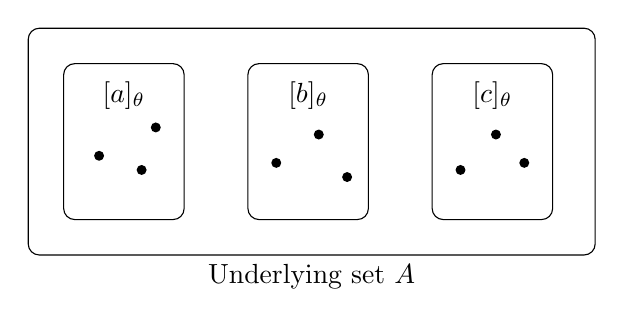
\begin{tikzpicture}[scale=0.9]
\draw[rounded corners] (0,0) rectangle (8,3.2);
\draw[rounded corners] (0.5,0.5) rectangle (2.2,2.7);
\draw[rounded corners] (3.1,0.5) rectangle (4.8,2.7);
\draw[rounded corners] (5.7,0.5) rectangle (7.4,2.7);

\node at (1.35,2.25) {\([a]_\theta\)};
\node at (3.95,2.25) {\([b]_\theta\)};
\node at (6.55,2.25) {\([c]_\theta\)};

\fill (1.0,1.4) circle (2pt);
\fill (1.6,1.2) circle (2pt);
\fill (1.8,1.8) circle (2pt);

\fill (3.5,1.3) circle (2pt);
\fill (4.1,1.7) circle (2pt);
\fill (4.5,1.1) circle (2pt);

\fill (6.1,1.2) circle (2pt);
\fill (6.6,1.7) circle (2pt);
\fill (7.0,1.3) circle (2pt);

\node[below] at (4,0) {Underlying set \(A\)};
\end{tikzpicture}
\end{center}

%%%%%%%%%%%%%%%%%%%%%%%%%%%%%%%%%%%%%%%%%%%%%%%%%%%%%%%%%%%%
\subsection{Quotient Algebras}
\label{subsec:quotient-algebras}
%%%%%%%%%%%%%%%%%%%%%%%%%%%%%%%%%%%%%%%%%%%%%%%%%%%%%%%%%%%%

\begin{definitionbox}{Quotient Algebra}
Let \(\theta\) be a congruence on \(\mathbf A\). The \emph{quotient algebra}
\(\mathbf A/\theta\) has underlying set \(A/\theta\), with operations defined
by
\[ f^{A/\theta}([a_1]_\theta,\ldots,[a_n]_\theta)
=[f^A(a_1,\ldots,a_n)]_\theta. \]
\end{definitionbox}

Compatibility of \(\theta\) ensures that the operation does not depend on
the chosen representatives.

%%%%%%%%%%%%%%%%%%%%%%%%%%%%%%%%%%%%%%%%%%%%%%%%%%%%%%%%%%%%
\subsection{Familiar Quotients as Congruence Quotients}
\label{subsec:familiar-congruence-quotients}
%%%%%%%%%%%%%%%%%%%%%%%%%%%%%%%%%%%%%%%%%%%%%%%%%%%%%%%%%%%%

The universal-algebra construction contains familiar quotient structures.

For groups, a normal subgroup \(N\trianglelefteq G\) determines

\[ a\mathrel{\theta_N}b
\iff a^{-1}b\in N. \]

Then

\[ G/\theta_N\cong G/N. \]

For rings, an ideal \(I\trianglelefteq R\) determines

\[ a\mathrel{\theta_I}b
\iff a-b\in I, \]

and

\[ R/\theta_I\cong R/I. \]

For modules, a submodule \(N\leq M\) determines

\[ x\mathrel{\theta_N}y
\iff x-y\in N. \]

Thus congruences provide the general mechanism behind algebraic quotients.

%%%%%%%%%%%%%%%%%%%%%%%%%%%%%%%%%%%%%%%%%%%%%%%%%%%%%%%%%%%%
\subsection{Kernels as Congruences}
\label{subsec:kernels-as-congruences}
%%%%%%%%%%%%%%%%%%%%%%%%%%%%%%%%%%%%%%%%%%%%%%%%%%%%%%%%%%%%

For a homomorphism

\[ h:\mathbf A\to\mathbf B, \]

define a relation on \(A\) by

\[ a\mathrel{\ker h}b
\iff h(a)=h(b). \]

Here \(\ker h\) denotes a relation rather than merely a subset.

\begin{theorem}[Kernel Congruence]
The relation
\[ a\mathrel{\ker h}b\iff h(a)=h(b) \]
is a congruence relation on \(\mathbf A\).
\end{theorem}

\begin{proof}
Equality in \(B\) is an equivalence relation, so \(\ker h\) is an
equivalence relation.

Suppose

\[ a_i\mathrel{\ker h}b_i \]

for \(i=1,\ldots,n\). Then

\[ h(a_i)=h(b_i). \]

Since \(h\) preserves \(f\),

\[
\begin{aligned}
h(f^A(a_1,\ldots,a_n))
&=f^B(h(a_1),\ldots,h(a_n))\\
&=f^B(h(b_1),\ldots,h(b_n))\\
&=h(f^A(b_1,\ldots,b_n)).
\end{aligned}
\]

Therefore

\[ f^A(a_1,\ldots,a_n)\mathrel{\ker h}f^A(b_1,\ldots,b_n). \]

Hence \(\ker h\) is compatible with every fundamental operation.
\end{proof}

%%%%%%%%%%%%%%%%%%%%%%%%%%%%%%%%%%%%%%%%%%%%%%%%%%%%%%%%%%%%
\subsection{First Isomorphism Theorem}
\label{subsec:universal-first-isomorphism}
%%%%%%%%%%%%%%%%%%%%%%%%%%%%%%%%%%%%%%%%%%%%%%%%%%%%%%%%%%%%

The familiar First Isomorphism Theorems for groups, rings, and modules are
instances of one general theorem.

\begin{theorem}[First Isomorphism Theorem for Universal Algebras]
Let
\[ h:\mathbf A\to\mathbf B \]
be a homomorphism. Then
\[ \mathbf A/\ker h\cong\Image(h). \]
\end{theorem}

The quotient identifies precisely those elements of \(A\) that \(h\) cannot
distinguish.

%%%%%%%%%%%%%%%%%%%%%%%%%%%%%%%%%%%%%%%%%%%%%%%%%%%%%%%%%%%%
\subsection{First Isomorphism Diagram}
\label{subsec:universal-first-isomorphism-diagram}
%%%%%%%%%%%%%%%%%%%%%%%%%%%%%%%%%%%%%%%%%%%%%%%%%%%%%%%%%%%%

\begin{center}
\begin{tikzcd}[column sep=large,row sep=large]
\mathbf A
\arrow[r,"h"]
\arrow[d,"\pi"']
&
\Image(h)
\\
\mathbf A/\ker h
\arrow[ur,"\overline h"',"\cong"]
\end{tikzcd}
\end{center}

The map

\[ \pi(a)=[a]_{\ker h} \]

is the quotient map.

The induced map is

\[ \overline h([a])=h(a). \]

The bar over \(h\) in \(\overline h\) is read ``\(h\) bar.''

%%%%%%%%%%%%%%%%%%%%%%%%%%%%%%%%%%%%%%%%%%%%%%%%%%%%%%%%%%%%
\subsection{Worked Example: A Congruence on the Integers}
\label{subsec:worked-congruence-integers}
%%%%%%%%%%%%%%%%%%%%%%%%%%%%%%%%%%%%%%%%%%%%%%%%%%%%%%%%%%%%

\begin{workedexamplebox}{Congruence Modulo \(n\)}

Consider the algebra

\[ \mathbf Z=(\Z,+,-,0). \]

Define

\[ a\mathrel{\theta}b
\iff a\equiv b\pmod n. \]

Show that \(\theta\) is compatible with addition.

\begin{tabularx}{\textwidth}{@{}>{\raggedright\arraybackslash}p{0.42\textwidth}X@{}}
Assume corresponding inputs are equivalent. &
\(a\equiv a'\pmod n,\quad b\equiv b'\pmod n\)\\
Rewrite using divisibility. &
\(n\mid(a-a'),\quad n\mid(b-b')\)\\
Add the differences. &
\(n\mid[(a+b)-(a'+b')]\)\\
Return to congruence notation. &
\(a+b\equiv a'+b'\pmod n\)
\end{tabularx}

\begin{answerbox}
\[ \boxed{a\mathrel{\theta}a',\ b\mathrel{\theta}b'
\Longrightarrow a+b\mathrel{\theta}a'+b'.} \]
\end{answerbox}
\end{workedexamplebox}

%%%%%%%%%%%%%%%%%%%%%%%%%%%%%%%%%%%%%%%%%%%%%%%%%%%%%%%%%%%%
\subsection{Direct Products}
\label{subsec:universal-direct-products}
%%%%%%%%%%%%%%%%%%%%%%%%%%%%%%%%%%%%%%%%%%%%%%%%%%%%%%%%%%%%

Let

\[ \mathbf A_i \]

be algebras of the same signature.

Their direct product has underlying set

\[ \prod_{i\in I}A_i. \]

The product symbol

\[ \prod \]

is the uppercase Greek letter pi used as a product operator and is read
``the product over \(i\) in \(I\).''

Operations are defined coordinatewise.

For an \(n\)-ary operation \(f\),

\[
f^{\prod A_i}
\left(
(a_{1i})_{i\in I},\ldots,(a_{ni})_{i\in I}
\right)
=
\left(
f^{A_i}(a_{1i},\ldots,a_{ni})
\right)_{i\in I}.
\]

%%%%%%%%%%%%%%%%%%%%%%%%%%%%%%%%%%%%%%%%%%%%%%%%%%%%%%%%%%%%
\subsection{Product Example}
\label{subsec:universal-product-example}
%%%%%%%%%%%%%%%%%%%%%%%%%%%%%%%%%%%%%%%%%%%%%%%%%%%%%%%%%%%%

For groups \(G\) and \(H\),

\[ (g_1,h_1)(g_2,h_2)
=(g_1g_2,h_1h_2). \]

For rings \(R\) and \(S\),

\[ (r_1,s_1)+(r_2,s_2)
=(r_1+r_2,s_1+s_2), \]

and

\[ (r_1,s_1)(r_2,s_2)
=(r_1r_2,s_1s_2). \]

These are both instances of the universal direct-product construction.

%%%%%%%%%%%%%%%%%%%%%%%%%%%%%%%%%%%%%%%%%%%%%%%%%%%%%%%%%%%%
\subsection{Homomorphic Images}
\label{subsec:homomorphic-images}
%%%%%%%%%%%%%%%%%%%%%%%%%%%%%%%%%%%%%%%%%%%%%%%%%%%%%%%%%%%%

If

\[ h:\mathbf A\to\mathbf B \]

is a surjective homomorphism, then \(\mathbf B\) is called a
\emph{homomorphic image} of \(\mathbf A\).

By the First Isomorphism Theorem,

\[ \mathbf B\cong\mathbf A/\ker h. \]

Thus homomorphic images and quotient algebras are closely connected.

%%%%%%%%%%%%%%%%%%%%%%%%%%%%%%%%%%%%%%%%%%%%%%%%%%%%%%%%%%%%
\subsection{The Three Fundamental Constructions}
\label{subsec:hsp-constructions}
%%%%%%%%%%%%%%%%%%%%%%%%%%%%%%%%%%%%%%%%%%%%%%%%%%%%%%%%%%%%

Three operations on classes of algebras are particularly important:

\begin{itemize}
    \item taking homomorphic images;
    \item taking subalgebras;
    \item taking direct products.
\end{itemize}

They are traditionally abbreviated

\[ \mathbf H,\qquad\mathbf S,\qquad\mathbf P. \]

Here:

\begin{itemize}
    \item \(\mathbf H\) means homomorphic images;
    \item \(\mathbf S\) means subalgebras;
    \item \(\mathbf P\) means products.
\end{itemize}

Together they produce the abbreviation

\[ \mathbf{HSP}. \]

This is read ``H-S-P.''

%%%%%%%%%%%%%%%%%%%%%%%%%%%%%%%%%%%%%%%%%%%%%%%%%%%%%%%%%%%%
\subsection{Varieties}
\label{subsec:universal-varieties}
%%%%%%%%%%%%%%%%%%%%%%%%%%%%%%%%%%%%%%%%%%%%%%%%%%%%%%%%%%%%

\begin{definitionbox}{Variety}
A \emph{variety} is a class of algebras of a fixed signature that can be
defined by a collection of identities.
\end{definitionbox}

Examples include:

\begin{itemize}
    \item groups;
    \item abelian groups;
    \item rings;
    \item commutative rings;
    \item lattices;
    \item distributive lattices;
    \item Boolean algebras.
\end{itemize}

Each is characterized by equations involving its fundamental operations.

%%%%%%%%%%%%%%%%%%%%%%%%%%%%%%%%%%%%%%%%%%%%%%%%%%%%%%%%%%%%
\subsection{Birkhoff's HSP Theorem}
\label{subsec:birkhoff-hsp}
%%%%%%%%%%%%%%%%%%%%%%%%%%%%%%%%%%%%%%%%%%%%%%%%%%%%%%%%%%%%

One of the central results of universal algebra characterizes varieties
structurally.

\begin{theorem}[Birkhoff's HSP Theorem]
A class of algebras of a fixed finitary signature is a variety if and only
if it is closed under:
\begin{itemize}
    \item homomorphic images;
    \item subalgebras;
    \item direct products.
\end{itemize}
\end{theorem}

Symbolically,

\[ \boxed{\text{equational class}\iff\text{HSP-closed class}.} \]

This theorem creates a deep bridge between syntax and structure.

%%%%%%%%%%%%%%%%%%%%%%%%%%%%%%%%%%%%%%%%%%%%%%%%%%%%%%%%%%%%
\subsection{Syntax Versus Structure}
\label{subsec:syntax-structure-universal}
%%%%%%%%%%%%%%%%%%%%%%%%%%%%%%%%%%%%%%%%%%%%%%%%%%%%%%%%%%%%

Birkhoff's theorem connects two viewpoints.

\begin{center}
\begin{tikzpicture}[
    node distance=28mm,
    box/.style={draw,rounded corners,align=center,inner sep=7pt},
    >=stealth
]
\node[box] (syntax) {Syntax\\identities\\\(s\approx t\)};
\node[box,right=of syntax] (structure) {Structure\\H, S, P\\constructions};

\draw[<->,thick] (syntax)--node[above]{Birkhoff's theorem}(structure);
\end{tikzpicture}
\end{center}

The left side describes algebras using equations.

The right side describes the same classes using closure properties.

This syntax--semantics relationship is one of the major themes connecting
universal algebra with mathematical logic.

%%%%%%%%%%%%%%%%%%%%%%%%%%%%%%%%%%%%%%%%%%%%%%%%%%%%%%%%%%%%
\subsection{Why Identities Survive HSP}
\label{subsec:identities-survive-hsp}
%%%%%%%%%%%%%%%%%%%%%%%%%%%%%%%%%%%%%%%%%%%%%%%%%%%%%%%%%%%%

Suppose an identity

\[ s\approx t \]

holds in an algebra.

It continues to hold in every subalgebra because the operations are
restrictions of the original operations.

It continues to hold in direct products because equations are evaluated
coordinatewise.

It also continues to hold in homomorphic images because homomorphisms
preserve term operations.

Thus equationally defined classes are automatically HSP-closed.

The difficult direction of Birkhoff's theorem shows that HSP closure is also
sufficient.

%%%%%%%%%%%%%%%%%%%%%%%%%%%%%%%%%%%%%%%%%%%%%%%%%%%%%%%%%%%%
\subsection{Equational Theories}
\label{subsec:equational-theories}
%%%%%%%%%%%%%%%%%%%%%%%%%%%%%%%%%%%%%%%%%%%%%%%%%%%%%%%%%%%%

For an algebra \(\mathbf A\), one may collect every identity true in
\(\mathbf A\).

This collection is called its \emph{equational theory}.

One may write

\[ \operatorname{Eq}(\mathbf A) \]

for the set of identities satisfied by \(\mathbf A\).

More generally, for a class \(\mathcal K\),

\[ \operatorname{Eq}(\mathcal K) \]

denotes the identities satisfied by every algebra in \(\mathcal K\).

The symbol

\[ \mathcal K \]

is a calligraphic capital \(K\), read simply ``script \(K\),'' and commonly
used to represent a class of structures.

%%%%%%%%%%%%%%%%%%%%%%%%%%%%%%%%%%%%%%%%%%%%%%%%%%%%%%%%%%%%
\subsection{Models of Identities}
\label{subsec:models-identities}
%%%%%%%%%%%%%%%%%%%%%%%%%%%%%%%%%%%%%%%%%%%%%%%%%%%%%%%%%%%%

Given a set \(E\) of identities, one may consider all algebras satisfying
them.

This class is often denoted

\[ \operatorname{Mod}(E). \]

It is read ``the models of \(E\).''

Thus there is a natural relationship

\[
\text{identities}
\longleftrightarrow
\text{classes of algebras}.
\]

This is an algebraic version of the broader logical relationship between
formal theories and their models.

%%%%%%%%%%%%%%%%%%%%%%%%%%%%%%%%%%%%%%%%%%%%%%%%%%%%%%%%%%%%
\subsection{Term Algebras}
\label{subsec:term-algebras}
%%%%%%%%%%%%%%%%%%%%%%%%%%%%%%%%%%%%%%%%%%%%%%%%%%%%%%%%%%%%

Terms themselves can be organized into an algebra.

Let

\[ X=\{x_1,x_2,\ldots\} \]

be a collection of variables.

The set of all \(\Sigma\)-terms in variables from \(X\) is denoted

\[ T_\Sigma(X). \]

This is read ``the term algebra over signature sigma on \(X\).''

Operations are defined formally by combining terms.

For example, if \(f\) is binary and \(s,t\) are terms, then

\[ f(s,t) \]

is another term.

%%%%%%%%%%%%%%%%%%%%%%%%%%%%%%%%%%%%%%%%%%%%%%%%%%%%%%%%%%%%
\subsection{Term Trees}
\label{subsec:term-trees}
%%%%%%%%%%%%%%%%%%%%%%%%%%%%%%%%%%%%%%%%%%%%%%%%%%%%%%%%%%%%

A term has an underlying tree structure.

For example,

\[ f(g(x),f(y,z)) \]

may be visualized as

\begin{center}
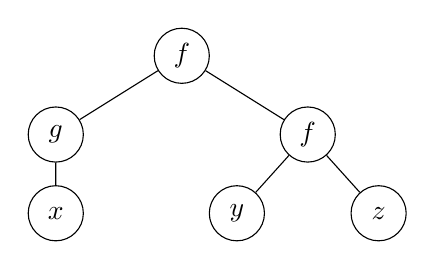
\begin{tikzpicture}[
    level distance=10mm,
    level 1/.style={sibling distance=32mm},
    level 2/.style={sibling distance=18mm},
    every node/.style={draw,circle,minimum size=7mm,inner sep=1pt},
    edge from parent/.style={draw,-}
]
\node {\(f\)}
    child {node {\(g\)}
        child {node {\(x\)}}}
    child {node {\(f\)}
        child {node {\(y\)}}
        child {node {\(z\)}}};
\end{tikzpicture}
\end{center}

The leaves are variables or constants.

Internal vertices represent operations.

This tree viewpoint is important in logic, computer algebra, and theoretical
computer science.

%%%%%%%%%%%%%%%%%%%%%%%%%%%%%%%%%%%%%%%%%%%%%%%%%%%%%%%%%%%%
\subsection{Free Algebras}
\label{subsec:free-algebras}
%%%%%%%%%%%%%%%%%%%%%%%%%%%%%%%%%%%%%%%%%%%%%%%%%%%%%%%%%%%%

A free algebra is generated by elements satisfying no relations other than
those required by the defining identities of its variety.

\begin{definitionbox}{Free Algebra}
Let \(\mathcal V\) be a variety and \(X\) a set. A \emph{free algebra} on
\(X\) is an algebra \(F_{\mathcal V}(X)\in\mathcal V\) equipped with a map
\[ \iota:X\to F_{\mathcal V}(X) \]
such that every function
\[ f:X\to A \]
into an algebra \(A\in\mathcal V\) extends uniquely to a homomorphism
\[ \widehat f:F_{\mathcal V}(X)\to A. \]
\end{definitionbox}

The symbol

\[ \widehat f \]

is read ``\(f\) hat.''

%%%%%%%%%%%%%%%%%%%%%%%%%%%%%%%%%%%%%%%%%%%%%%%%%%%%%%%%%%%%
\subsection{Universal Property of a Free Algebra}
\label{subsec:free-algebra-universal-property}
%%%%%%%%%%%%%%%%%%%%%%%%%%%%%%%%%%%%%%%%%%%%%%%%%%%%%%%%%%%%

The defining property is represented by

\begin{center}
\begin{tikzcd}[column sep=large,row sep=large]
X
\arrow[r,"\iota"]
\arrow[dr,"f"']
&
F_{\mathcal V}(X)
\arrow[d,dashed,"\widehat f"]
\\
&
A
\end{tikzcd}
\end{center}

The dashed arrow exists uniquely.

This is called a \emph{universal property}.

It characterizes the free algebra structurally rather than through a
particular construction.

%%%%%%%%%%%%%%%%%%%%%%%%%%%%%%%%%%%%%%%%%%%%%%%%%%%%%%%%%%%%
\subsection{Examples of Free Algebras}
\label{subsec:free-algebra-examples}
%%%%%%%%%%%%%%%%%%%%%%%%%%%%%%%%%%%%%%%%%%%%%%%%%%%%%%%%%%%%

Several familiar constructions are free objects.

The free group on a set \(X\) is the group generated by \(X\) with no
relations beyond the group axioms.

The free abelian group on \(n\) generators is

\[ \Z^n. \]

The free vector space over a field \(F\) on \(n\) generators is

\[ F^n. \]

The polynomial ring

\[ R[x_1,\ldots,x_n] \]

has an important free universal property as a commutative \(R\)-algebra.

Thus ``free'' is a recurring structural idea across algebra.

%%%%%%%%%%%%%%%%%%%%%%%%%%%%%%%%%%%%%%%%%%%%%%%%%%%%%%%%%%%%
\subsection{Presentations by Generators and Relations}
\label{subsec:universal-presentations}
%%%%%%%%%%%%%%%%%%%%%%%%%%%%%%%%%%%%%%%%%%%%%%%%%%%%%%%%%%%%

An algebra can often be described by starting with a free algebra and then
imposing relations.

Schematically,

\[ \boxed{\text{generators}+\text{relations}
\longrightarrow\text{presented algebra}.} \]

If \(F(X)\) is free and \(\theta\) is the congruence generated by the desired
relations, then the presented algebra has the form

\[ F(X)/\theta. \]

This generalizes group presentations, quotient rings, and module
presentations.

%%%%%%%%%%%%%%%%%%%%%%%%%%%%%%%%%%%%%%%%%%%%%%%%%%%%%%%%%%%%
\subsection{Congruence Generated by Relations}
\label{subsec:generated-congruence}
%%%%%%%%%%%%%%%%%%%%%%%%%%%%%%%%%%%%%%%%%%%%%%%%%%%%%%%%%%%%

Suppose

\[ R\subseteq A\times A \]

is a collection of pairs that one wishes to declare equivalent.

There exists a smallest congruence containing \(R\).

It may be denoted

\[ \operatorname{Cg}(R). \]

This is read ``the congruence generated by \(R\).''

Thus presentations can be written abstractly as

\[ F(X)/\operatorname{Cg}(R). \]

%%%%%%%%%%%%%%%%%%%%%%%%%%%%%%%%%%%%%%%%%%%%%%%%%%%%%%%%%%%%
\subsection{Worked Example: A Presented Algebra}
\label{subsec:worked-presented-algebra}
%%%%%%%%%%%%%%%%%%%%%%%%%%%%%%%%%%%%%%%%%%%%%%%%%%%%%%%%%%%%

\begin{workedexamplebox}{A Cyclic Group as a Quotient}

Start with the free group on one generator \(x\).

Impose the relation

\[ x^n=e. \]

\begin{tabularx}{\textwidth}{@{}>{\raggedright\arraybackslash}p{0.42\textwidth}X@{}}
Begin with the free group. & \(F(x)\cong\Z\)\\
Impose the relation. & \(x^n=e\)\\
Generate the corresponding congruence. &
Identify powers whose exponents differ by multiples of \(n\).\\
Take the quotient. & \(F(x)/\operatorname{Cg}(x^n,e)\)
\end{tabularx}

\begin{answerbox}
\[ \boxed{F(x)/\operatorname{Cg}(x^n,e)\cong\Z/n\Z.} \]
\end{answerbox}
\end{workedexamplebox}

%%%%%%%%%%%%%%%%%%%%%%%%%%%%%%%%%%%%%%%%%%%%%%%%%%%%%%%%%%%%
\subsection{Congruence Lattices}
\label{subsec:congruence-lattices}
%%%%%%%%%%%%%%%%%%%%%%%%%%%%%%%%%%%%%%%%%%%%%%%%%%%%%%%%%%%%

The congruence relations on an algebra are naturally ordered by inclusion.

Let

\[ \operatorname{Con}(\mathbf A) \]

denote the set of all congruences on \(\mathbf A\).

This is read ``the congruence lattice of \(\mathbf A\).''

The smallest congruence is equality:

\[ \Delta_A=\{(a,a):a\in A\}. \]

The uppercase Greek letter

\[ \Delta \]

is delta, pronounced ``DEL-tuh.''

Here \(\Delta_A\) denotes the diagonal or equality relation.

The largest congruence is

\[ \nabla_A=A\times A. \]

The symbol

\[ \nabla \]

is called \emph{nabla}, pronounced ``NAB-luh.''

Here it denotes the universal relation in which every pair is equivalent.

%%%%%%%%%%%%%%%%%%%%%%%%%%%%%%%%%%%%%%%%%%%%%%%%%%%%%%%%%%%%
\subsection{The Congruence Lattice}
\label{subsec:congruence-lattice-structure}
%%%%%%%%%%%%%%%%%%%%%%%%%%%%%%%%%%%%%%%%%%%%%%%%%%%%%%%%%%%%

Under inclusion,

\[ \operatorname{Con}(\mathbf A) \]

forms a lattice.

For a small algebra, its structure may resemble

\begin{center}
\begin{tikzpicture}[
    node distance=12mm and 18mm,
    every node/.style={draw,circle,inner sep=2pt,minimum size=9mm}
]
\node (top) {\(\nabla_A\)};
\node[below left=of top] (a) {\(\alpha\)};
\node[below right=of top] (b) {\(\beta\)};
\node[below=22mm of top] (bottom) {\(\Delta_A\)};

\draw (top)--(a);
\draw (top)--(b);
\draw (a)--(bottom);
\draw (b)--(bottom);
\end{tikzpicture}
\end{center}

The letters

\[ \alpha,\qquad\beta \]

are the lowercase Greek letters alpha and beta, pronounced ``AL-fuh'' and
``BAY-tuh.''

They are commonly used to denote congruence relations.

The full theory of lattices is developed canonically in
\cref{sec:lattice-theory}.

%%%%%%%%%%%%%%%%%%%%%%%%%%%%%%%%%%%%%%%%%%%%%%%%%%%%%%%%%%%%
\subsection{Congruence-Simple Algebras}
\label{subsec:congruence-simple}
%%%%%%%%%%%%%%%%%%%%%%%%%%%%%%%%%%%%%%%%%%%%%%%%%%%%%%%%%%%%

\begin{definitionbox}{Simple Algebra}
An algebra \(\mathbf A\) is \emph{simple} if its only congruences are
\[ \Delta_A\qquad\text{and}\qquad\nabla_A. \]
\end{definitionbox}

This generalizes familiar notions of simplicity.

For example, simple groups have no nontrivial normal subgroups because
normal subgroups correspond to group congruences.

%%%%%%%%%%%%%%%%%%%%%%%%%%%%%%%%%%%%%%%%%%%%%%%%%%%%%%%%%%%%
\subsection{Subdirect Products}
\label{subsec:subdirect-products}
%%%%%%%%%%%%%%%%%%%%%%%%%%%%%%%%%%%%%%%%%%%%%%%%%%%%%%%%%%%%

Universal algebra also studies algebras embedded into products.

\begin{definitionbox}{Subdirect Product}
A subalgebra
\[ \mathbf A\leq\prod_{i\in I}\mathbf A_i \]
is a \emph{subdirect product} if every coordinate projection
\[ \pi_i:\mathbf A\to\mathbf A_i \]
is surjective.
\end{definitionbox}

Thus a subdirect product is simultaneously:

\begin{itemize}
    \item a subalgebra of a direct product;
    \item large enough to project onto every factor.
\end{itemize}

%%%%%%%%%%%%%%%%%%%%%%%%%%%%%%%%%%%%%%%%%%%%%%%%%%%%%%%%%%%%
\subsection{Subdirect Representation}
\label{subsec:subdirect-representation}
%%%%%%%%%%%%%%%%%%%%%%%%%%%%%%%%%%%%%%%%%%%%%%%%%%%%%%%%%%%%

Subdirect products allow complicated algebras to be represented using
simpler factors.

Schematically,

\begin{center}
\begin{tikzpicture}[
    node distance=12mm and 18mm,
    box/.style={draw,rounded corners,align=center,inner sep=5pt},
    >=stealth
]
\node[box] (A) {\(\mathbf A\)};
\node[box,below=of A] (prod)
{\(\mathbf A_1\times\mathbf A_2\times\cdots\)};
\node[box,below left=of prod] (A1) {\(\mathbf A_1\)};
\node[box,below right=of prod] (A2) {\(\mathbf A_2\)};

\draw[->,hook] (A)--(prod);
\draw[->] (A)--(A1);
\draw[->] (A)--(A2);
\end{tikzpicture}
\end{center}

This viewpoint leads to important representation theorems in universal
algebra.

%%%%%%%%%%%%%%%%%%%%%%%%%%%%%%%%%%%%%%%%%%%%%%%%%%%%%%%%%%%%
\subsection{Birkhoff's Subdirect Representation Theorem}
\label{subsec:birkhoff-subdirect}
%%%%%%%%%%%%%%%%%%%%%%%%%%%%%%%%%%%%%%%%%%%%%%%%%%%%%%%%%%%%

A major structural result states, roughly, that algebras can be built from
subdirectly irreducible pieces.

\begin{theorem}[Subdirect Representation Theorem]
Every algebra is isomorphic to a subdirect product of subdirectly
irreducible algebras.
\end{theorem}

This plays a role analogous to decomposition principles appearing elsewhere
in algebra.

A full proof requires a deeper study of congruence lattices and is deferred.

%%%%%%%%%%%%%%%%%%%%%%%%%%%%%%%%%%%%%%%%%%%%%%%%%%%%%%%%%%%%
\subsection{Unary Algebras}
\label{subsec:unary-algebras}
%%%%%%%%%%%%%%%%%%%%%%%%%%%%%%%%%%%%%%%%%%%%%%%%%%%%%%%%%%%%

A universal algebra may have only unary operations.

For example,

\[ \mathbf A=(A,f) \]

with

\[ f:A\to A \]

is a unary algebra.

Such structures can be represented by directed graphs in which every
element has an arrow to its image.

For example, if

\[ f(1)=2,\qquad f(2)=3,\qquad f(3)=3, \]

then

\begin{center}
\begin{tikzpicture}[
    node distance=18mm,
    every node/.style={draw,circle,minimum size=8mm},
    >=stealth
]
\node (one) {\(1\)};
\node[right=of one] (two) {\(2\)};
\node[right=of two] (three) {\(3\)};

\draw[->] (one)--(two);
\draw[->] (two)--(three);
\draw[->] (three) edge[loop right] (three);
\end{tikzpicture}
\end{center}

Universal algebra therefore includes structures much more general than
groups and rings.

%%%%%%%%%%%%%%%%%%%%%%%%%%%%%%%%%%%%%%%%%%%%%%%%%%%%%%%%%%%%
\subsection{Semilattices}
\label{subsec:universal-semilattices}
%%%%%%%%%%%%%%%%%%%%%%%%%%%%%%%%%%%%%%%%%%%%%%%%%%%%%%%%%%%%

A \emph{semilattice} provides a simple but important example of an
equational class.

A meet-semilattice has one binary operation \(\wedge\) satisfying

\[ x\wedge(y\wedge z)\approx(x\wedge y)\wedge z, \]

\[ x\wedge y\approx y\wedge x, \]

and

\[ x\wedge x\approx x. \]

Thus a semilattice is characterized by associativity, commutativity, and
idempotence.

Its deeper order-theoretic interpretation belongs to lattice theory.

%%%%%%%%%%%%%%%%%%%%%%%%%%%%%%%%%%%%%%%%%%%%%%%%%%%%%%%%%%%%
\subsection{Boolean Algebras}
\label{subsec:universal-boolean-algebras}
%%%%%%%%%%%%%%%%%%%%%%%%%%%%%%%%%%%%%%%%%%%%%%%%%%%%%%%%%%%%

Boolean algebras provide another important variety.

A common signature contains

\[ \wedge,\qquad\vee,\qquad\neg,\qquad0,\qquad1. \]

The symbol

\[ \neg \]

is read ``not'' or ``complement'' depending on context.

Boolean algebra identities abstract the familiar operations of intersection,
union, complement, the empty set, and the universal set.

They also model propositional logic.

This demonstrates how the same equational structure may have several
different interpretations.

%%%%%%%%%%%%%%%%%%%%%%%%%%%%%%%%%%%%%%%%%%%%%%%%%%%%%%%%%%%%
\subsection{One Algebraic Pattern, Many Models}
\label{subsec:one-pattern-many-models}
%%%%%%%%%%%%%%%%%%%%%%%%%%%%%%%%%%%%%%%%%%%%%%%%%%%%%%%%%%%%

Boolean algebra illustrates the universal-algebra philosophy particularly
well.

\begin{center}
\begin{tikzpicture}[
    node distance=10mm and 15mm,
    box/.style={draw,rounded corners,align=center,inner sep=5pt},
    >=stealth
]
\node[box] (bool) {Boolean algebra\\identities};
\node[box,below left=of bool] (sets) {Sets\\\(\cap,\cup,{}^c\)};
\node[box,below=of bool] (logic) {Logic\\AND, OR, NOT};
\node[box,below right=of bool] (bits) {Binary values\\\(0,1\)};

\draw[->] (bool)--(sets);
\draw[->] (bool)--(logic);
\draw[->] (bool)--(bits);
\end{tikzpicture}
\end{center}

The underlying objects differ, but the same identities govern all of them.

%%%%%%%%%%%%%%%%%%%%%%%%%%%%%%%%%%%%%%%%%%%%%%%%%%%%%%%%%%%%
\subsection{Polynomials in Universal Algebra}
\label{subsec:universal-polynomials}
%%%%%%%%%%%%%%%%%%%%%%%%%%%%%%%%%%%%%%%%%%%%%%%%%%%%%%%%%%%%

Universal algebra generalizes the notion of polynomial beyond ordinary
rings.

Starting with fundamental operations and allowing fixed elements of an
algebra as parameters produces \emph{polynomial operations}.

For example, in a group, expressions such as

\[ axb^{-1}x^{-1} \]

define polynomial-like operations in the universal-algebraic sense.

Thus the word ``polynomial'' can refer to formal combinations of the
available algebraic operations, not merely powers and coefficients in a
ring.

%%%%%%%%%%%%%%%%%%%%%%%%%%%%%%%%%%%%%%%%%%%%%%%%%%%%%%%%%%%%
\subsection{Clones of Operations}
\label{subsec:clones-preview}
%%%%%%%%%%%%%%%%%%%%%%%%%%%%%%%%%%%%%%%%%%%%%%%%%%%%%%%%%%%%

The term operations of an algebra can themselves be studied collectively.

A collection of finitary operations containing projections and closed under
composition is called a \emph{clone}.

For example, the projection

\[ \pi_i^n(x_1,\ldots,x_n)=x_i \]

returns the \(i\)th input.

Clone theory provides another way to study algebraic structures through the
operations they generate.

A full treatment belongs to more specialized universal algebra.

%%%%%%%%%%%%%%%%%%%%%%%%%%%%%%%%%%%%%%%%%%%%%%%%%%%%%%%%%%%%
\subsection{Universal Algebra and Logic}
\label{subsec:universal-algebra-logic}
%%%%%%%%%%%%%%%%%%%%%%%%%%%%%%%%%%%%%%%%%%%%%%%%%%%%%%%%%%%%

Universal algebra has a strong logical component.

An identity

\[ s\approx t \]

can be interpreted as the universally quantified statement

\[ \forall x_1\cdots\forall x_n,\quad s=t. \]

Thus equational logic is a restricted but powerful fragment of first-order
logic.

Universal algebra studies what can be concluded from such equations and how
those conclusions correspond to structural properties of algebras.

%%%%%%%%%%%%%%%%%%%%%%%%%%%%%%%%%%%%%%%%%%%%%%%%%%%%%%%%%%%%
\subsection{Equational Consequence}
\label{subsec:equational-consequence}
%%%%%%%%%%%%%%%%%%%%%%%%%%%%%%%%%%%%%%%%%%%%%%%%%%%%%%%%%%%%

Suppose \(E\) is a collection of identities.

If every algebra satisfying \(E\) also satisfies

\[ s\approx t, \]

then \(s\approx t\) is an \emph{equational consequence} of \(E\).

One may write

\[ E\models s\approx t. \]

The symbol

\[ \models \]

is called the semantic consequence symbol and is commonly read
``models'' or ``semantically entails.''

Thus

\[ E\models s\approx t \]

means ``every model of \(E\) satisfies the identity \(s\approx t\).''

%%%%%%%%%%%%%%%%%%%%%%%%%%%%%%%%%%%%%%%%%%%%%%%%%%%%%%%%%%%%
\subsection{Formal Derivation of Identities}
\label{subsec:formal-equational-derivation}
%%%%%%%%%%%%%%%%%%%%%%%%%%%%%%%%%%%%%%%%%%%%%%%%%%%%%%%%%%%%

Identities can also be manipulated syntactically using rules such as:

\begin{itemize}
    \item reflexivity;
    \item symmetry;
    \item transitivity;
    \item substitution;
    \item compatibility with operations.
\end{itemize}

A formally derivable identity may be written

\[ E\vdash s\approx t. \]

The symbol

\[ \vdash \]

is called the turnstile and is read ``proves'' or ``syntactically entails.''

The distinction is:

\[ \vdash\quad\text{syntactic derivation}, \qquad
\models\quad\text{semantic consequence}. \]

%%%%%%%%%%%%%%%%%%%%%%%%%%%%%%%%%%%%%%%%%%%%%%%%%%%%%%%%%%%%
\subsection{Completeness of Equational Logic}
\label{subsec:equational-completeness}
%%%%%%%%%%%%%%%%%%%%%%%%%%%%%%%%%%%%%%%%%%%%%%%%%%%%%%%%%%%%

A fundamental result states that semantic and syntactic consequence agree
for identities.

\begin{theorem}[Completeness of Equational Logic]
For a set \(E\) of identities,
\[ E\vdash s\approx t
\quad\Longleftrightarrow\quad
E\models s\approx t. \]
\end{theorem}

Thus an identity is true in every algebra satisfying \(E\) precisely when it
can be formally derived from \(E\) using the rules of equational logic.

%%%%%%%%%%%%%%%%%%%%%%%%%%%%%%%%%%%%%%%%%%%%%%%%%%%%%%%%%%%%
\subsection{Worked Example: Deriving an Identity}
\label{subsec:worked-equational-identity}
%%%%%%%%%%%%%%%%%%%%%%%%%%%%%%%%%%%%%%%%%%%%%%%%%%%%%%%%%%%%

\begin{workedexamplebox}{Uniqueness from Equational Laws}

Suppose a binary operation satisfies

\[ x\cdot e\approx x,\qquad x\cdot x^{-1}\approx e. \]

Evaluate

\[ (x\cdot x^{-1})\cdot e. \]

\begin{tabularx}{\textwidth}{@{}>{\raggedright\arraybackslash}p{0.42\textwidth}X@{}}
Apply the inverse identity. &
\((x\cdot x^{-1})\cdot e=e\cdot e\)\\
Apply the identity law with \(x=e\). &
\(e\cdot e=e\)
\end{tabularx}

\begin{answerbox}
\[ \boxed{(x\cdot x^{-1})\cdot e\approx e.} \]
\end{answerbox}
\end{workedexamplebox}

%%%%%%%%%%%%%%%%%%%%%%%%%%%%%%%%%%%%%%%%%%%%%%%%%%%%%%%%%%%%
\subsection{Mal'cev Conditions: A Preview}
\label{subsec:malcev-preview}
%%%%%%%%%%%%%%%%%%%%%%%%%%%%%%%%%%%%%%%%%%%%%%%%%%%%%%%%%%%%

Some structural properties of entire varieties can themselves be
characterized by the existence of special terms.

One famous example uses a ternary term

\[ p(x,y,z) \]

satisfying

\[ p(x,x,z)\approx z,\qquad p(x,y,y)\approx x. \]

Such a term is called a \emph{Mal'cev term}.

The existence of a Mal'cev term implies strong properties of congruences,
including congruence permutability.

Groups provide the standard example:

\[ p(x,y,z)=xy^{-1}z. \]

Indeed,

\[ p(x,x,z)=xx^{-1}z=z, \]

and

\[ p(x,y,y)=xy^{-1}y=x. \]

%%%%%%%%%%%%%%%%%%%%%%%%%%%%%%%%%%%%%%%%%%%%%%%%%%%%%%%%%%%%
\subsection{Congruence Permutability}
\label{subsec:congruence-permutability}
%%%%%%%%%%%%%%%%%%%%%%%%%%%%%%%%%%%%%%%%%%%%%%%%%%%%%%%%%%%%

Given relations \(\alpha\) and \(\beta\), their relational compositions are

\[ \alpha\circ\beta
\qquad\text{and}\qquad
\beta\circ\alpha. \]

A variety is \emph{congruence permutable} if

\[ \alpha\circ\beta=\beta\circ\alpha \]

for every pair of congruences on every algebra in the variety.

Groups have this property.

This demonstrates a major theme of advanced universal algebra:

\begin{conceptbox}
Special algebraic terms can control global structural properties of
congruence lattices throughout an entire variety.
\end{conceptbox}

%%%%%%%%%%%%%%%%%%%%%%%%%%%%%%%%%%%%%%%%%%%%%%%%%%%%%%%%%%%%
\subsection{Congruence Distributivity: A Preview}
\label{subsec:congruence-distributivity-preview}
%%%%%%%%%%%%%%%%%%%%%%%%%%%%%%%%%%%%%%%%%%%%%%%%%%%%%%%%%%%%

A variety is called \emph{congruence distributive} when every congruence
lattice

\[ \operatorname{Con}(\mathbf A) \]

is distributive.

There are term conditions characterizing this property as well.

The detailed theory of such conditions belongs to advanced universal
algebra and connects strongly with lattice theory.

%%%%%%%%%%%%%%%%%%%%%%%%%%%%%%%%%%%%%%%%%%%%%%%%%%%%%%%%%%%%
\subsection{Locally Finite Varieties}
\label{subsec:locally-finite-varieties}
%%%%%%%%%%%%%%%%%%%%%%%%%%%%%%%%%%%%%%%%%%%%%%%%%%%%%%%%%%%%

\begin{definitionbox}{Locally Finite Variety}
A variety is \emph{locally finite} if every finitely generated algebra in
the variety is finite.
\end{definitionbox}

This property is important when studying finite algebraic structures and
computational questions.

For example, some varieties generated by finite algebras are locally finite,
while others are not.

%%%%%%%%%%%%%%%%%%%%%%%%%%%%%%%%%%%%%%%%%%%%%%%%%%%%%%%%%%%%
\subsection{The Variety Generated by an Algebra}
\label{subsec:variety-generated-algebra}
%%%%%%%%%%%%%%%%%%%%%%%%%%%%%%%%%%%%%%%%%%%%%%%%%%%%%%%%%%%%

Given an algebra \(\mathbf A\), the smallest variety containing it is
denoted

\[ \mathsf V(\mathbf A). \]

This is read ``the variety generated by \(\mathbf A\).''

By Birkhoff's theorem,

\[ \mathsf V(\mathbf A)=\mathbf{HSP}(\mathbf A), \]

where arbitrary repeated applications of homomorphic images, subalgebras,
and products are understood.

%%%%%%%%%%%%%%%%%%%%%%%%%%%%%%%%%%%%%%%%%%%%%%%%%%%%%%%%%%%%
\subsection{Universal Algebra and Category Theory}
\label{subsec:universal-algebra-category}
%%%%%%%%%%%%%%%%%%%%%%%%%%%%%%%%%%%%%%%%%%%%%%%%%%%%%%%%%%%%

Fix a signature \(\Sigma\).

Its algebras and homomorphisms form a category.

Schematically,

\begin{center}
\begin{tikzpicture}[
    node distance=12mm,
    box/.style={draw,rounded corners,align=center,inner sep=5pt},
    >=stealth
]
\node[box] (objects) {\(\Sigma\)-algebras\\objects};
\node[box,right=of objects] (maps) {Homomorphisms\\morphisms};
\node[box,right=of maps] (cat) {Category\\\(\mathbf{Alg}_\Sigma\)};

\draw[->] (objects)--(cat);
\draw[->] (maps)--(cat);
\end{tikzpicture}
\end{center}

Products and free algebras can then be characterized through universal
properties.

The full categorical language is developed canonically in
\cref{sec:category-theory}.

%%%%%%%%%%%%%%%%%%%%%%%%%%%%%%%%%%%%%%%%%%%%%%%%%%%%%%%%%%%%
\subsection{Universal Algebra and Computer Science}
\label{subsec:universal-algebra-computer-science}
%%%%%%%%%%%%%%%%%%%%%%%%%%%%%%%%%%%%%%%%%%%%%%%%%%%%%%%%%%%%

Universal algebra appears naturally in theoretical computer science.

Terms behave like syntax trees.

Operations behave like constructors.

Equations describe when different expressions should represent the same
object.

Applications include:

\begin{itemize}
    \item algebraic specification;
    \item term rewriting;
    \item automated theorem proving;
    \item programming-language semantics;
    \item constraint satisfaction problems;
    \item database theory.
\end{itemize}

The close relationship between syntax, operations, and equations makes
universal algebra particularly suitable for computational reasoning.

%%%%%%%%%%%%%%%%%%%%%%%%%%%%%%%%%%%%%%%%%%%%%%%%%%%%%%%%%%%%
\subsection{Universal Algebra and Constraint Satisfaction}
\label{subsec:universal-algebra-csp}
%%%%%%%%%%%%%%%%%%%%%%%%%%%%%%%%%%%%%%%%%%%%%%%%%%%%%%%%%%%%

A modern application of universal algebra occurs in the study of
\emph{constraint satisfaction problems}, often abbreviated CSPs.

The computational complexity of many CSPs can be analyzed using operations
that preserve the underlying relations.

These operations are called \emph{polymorphisms}.

This connection has made universal algebra an important tool in theoretical
computer science.

A complete treatment requires substantial additional material and is beyond
the scope of this introductory section.

%%%%%%%%%%%%%%%%%%%%%%%%%%%%%%%%%%%%%%%%%%%%%%%%%%%%%%%%%%%%
\subsection{Universal Algebra as a Unifying Language}
\label{subsec:universal-algebra-unifying-language}
%%%%%%%%%%%%%%%%%%%%%%%%%%%%%%%%%%%%%%%%%%%%%%%%%%%%%%%%%%%%

Many familiar concepts align under universal algebra.

\begin{center}
\begin{tabularx}{0.96\textwidth}{@{}lXXX@{}}
\toprule
\textbf{Universal Algebra} & \textbf{Groups} & \textbf{Rings} & \textbf{Modules}\\
\midrule
subalgebra & subgroup & subring & submodule\\
congruence & normal subgroup relation & ideal relation & submodule relation\\
quotient algebra & quotient group & quotient ring & quotient module\\
homomorphism & group homomorphism & ring homomorphism & module homomorphism\\
free algebra & free group & free ring/algebra & free module\\
product & direct product & product ring & product module\\
\bottomrule
\end{tabularx}
\end{center}

This table captures one of the main purposes of the subject: results that
look separate in individual algebra courses are often manifestations of a
single universal theorem.

%%%%%%%%%%%%%%%%%%%%%%%%%%%%%%%%%%%%%%%%%%%%%%%%%%%%%%%%%%%%
\subsection{A Structural Roadmap}
\label{subsec:universal-algebra-roadmap}
%%%%%%%%%%%%%%%%%%%%%%%%%%%%%%%%%%%%%%%%%%%%%%%%%%%%%%%%%%%%

The main ideas of universal algebra fit together as follows.

\begin{center}
\begin{tikzpicture}[
    node distance=8mm and 11mm,
    box/.style={draw,rounded corners,align=center,inner sep=4pt,font=\small},
    >=stealth
]
\node[box] (sig) {Signature};
\node[box,below=of sig] (alg) {Algebras};
\node[box,below left=of alg] (sub) {Subalgebras};
\node[box,below=of alg] (hom) {Homomorphisms};
\node[box,below right=of alg] (prod) {Products};
\node[box,below=of hom] (cong) {Congruences};
\node[box,below=of cong] (quot) {Quotients};
\node[box,below=of quot] (hsp) {HSP};
\node[box,below=of hsp] (var) {Varieties};
\node[box,below left=of var] (free) {Free algebras};
\node[box,below right=of var] (logic) {Equational logic};

\draw[->] (sig)--(alg);
\draw[->] (alg)--(sub);
\draw[->] (alg)--(hom);
\draw[->] (alg)--(prod);
\draw[->] (hom)--(cong);
\draw[->] (cong)--(quot);
\draw[->] (sub)--(hsp);
\draw[->] (quot)--(hsp);
\draw[->] (prod)--(hsp);
\draw[->] (hsp)--(var);
\draw[->] (var)--(free);
\draw[->] (var)--(logic);
\end{tikzpicture}
\end{center}

%%%%%%%%%%%%%%%%%%%%%%%%%%%%%%%%%%%%%%%%%%%%%%%%%%%%%%%%%%%%
\subsection{Common Errors}
\label{subsec:universal-algebra-common-errors}
%%%%%%%%%%%%%%%%%%%%%%%%%%%%%%%%%%%%%%%%%%%%%%%%%%%%%%%%%%%%

\subsubsection{Assuming Every Algebra Has Addition and Multiplication}

An algebra in universal algebra may have any specified collection of
finitary operations.

It need not resemble a ring.

%%%%%%%%%%%%%%%%%%%%%%%%%%%%%%%%%%%%%%%%%%%%%%%%%%%%%%%%%%%%
\subsubsection{Confusing an Operation Symbol with Its Interpretation}

The symbol \(f\) belongs to the signature.

The function

\[ f^A:A^n\to A \]

is its interpretation in the algebra \(\mathbf A\).

Different algebras of the same signature may interpret \(f\) differently.

%%%%%%%%%%%%%%%%%%%%%%%%%%%%%%%%%%%%%%%%%%%%%%%%%%%%%%%%%%%%
\subsubsection{Ignoring Arity}

Operation symbols come with fixed arities.

A binary operation cannot suddenly be interpreted as a unary operation in
another algebra of the same signature.

%%%%%%%%%%%%%%%%%%%%%%%%%%%%%%%%%%%%%%%%%%%%%%%%%%%%%%%%%%%%
\subsubsection{Assuming Any Equivalence Relation Gives a Quotient Algebra}

An equivalence relation must be compatible with every fundamental operation.

Only then is it a congruence.

%%%%%%%%%%%%%%%%%%%%%%%%%%%%%%%%%%%%%%%%%%%%%%%%%%%%%%%%%%%%
\subsubsection{Confusing Congruences with Subalgebras}

A subalgebra is a subset closed under operations.

A congruence is a compatible equivalence relation.

They play different structural roles.

%%%%%%%%%%%%%%%%%%%%%%%%%%%%%%%%%%%%%%%%%%%%%%%%%%%%%%%%%%%%
\subsubsection{Thinking the Kernel Must Be a Subset}

For group or ring homomorphisms, the kernel is commonly represented by a
special subset.

In general universal algebra, the natural kernel is the relation

\[ a\mathrel{\ker h}b\iff h(a)=h(b). \]

%%%%%%%%%%%%%%%%%%%%%%%%%%%%%%%%%%%%%%%%%%%%%%%%%%%%%%%%%%%%
\subsubsection{Assuming Every Class of Algebras Is a Variety}

A variety must be definable by identities.

Equivalently, by Birkhoff's theorem, it must satisfy the appropriate HSP
closure conditions.

%%%%%%%%%%%%%%%%%%%%%%%%%%%%%%%%%%%%%%%%%%%%%%%%%%%%%%%%%%%%
\subsubsection{Confusing an Identity with an Equation to Solve}

The expression

\[ xy\approx yx \]

means that commutativity holds for every pair of elements.

It is not asking for particular \(x\) and \(y\) satisfying the equation.

%%%%%%%%%%%%%%%%%%%%%%%%%%%%%%%%%%%%%%%%%%%%%%%%%%%%%%%%%%%%
\subsubsection{Confusing \(\models\) and \(\vdash\)}

The notation

\[ E\models s\approx t \]

refers to truth in all models.

The notation

\[ E\vdash s\approx t \]

refers to formal derivability.

Completeness tells us these agree for equational logic, but their meanings
are conceptually distinct.

%%%%%%%%%%%%%%%%%%%%%%%%%%%%%%%%%%%%%%%%%%%%%%%%%%%%%%%%%%%%
\subsubsection{Assuming Free Means No Axioms}

A free algebra in a variety still satisfies every identity defining that
variety.

``Free'' means that no additional relations among the generators are
imposed.

%%%%%%%%%%%%%%%%%%%%%%%%%%%%%%%%%%%%%%%%%%%%%%%%%%%%%%%%%%%%
\subsection{Applications}
\label{subsec:universal-algebra-applications}
%%%%%%%%%%%%%%%%%%%%%%%%%%%%%%%%%%%%%%%%%%%%%%%%%%%%%%%%%%%%

\begin{applicationbox}
\textbf{Abstract Algebra.}
Universal algebra explains why groups, rings, modules, lattices, and many
other structures possess parallel theories of subobjects, quotients,
homomorphisms, and products.

\medskip

\textbf{Lattice Theory.}
The congruences of an algebra form a lattice, making lattice theory a major
tool for studying algebraic structure.

\medskip

\textbf{Mathematical Logic.}
Identities and varieties provide a concrete setting for studying the
relationship between formal syntax and mathematical models.

\medskip

\textbf{Category Theory.}
Algebras of a fixed signature form categories, and free algebras are
characterized by universal properties.

\medskip

\textbf{Computer Science.}
Term algebras, equations, and free structures appear in algebraic
specification, rewriting systems, programming-language semantics, and
automated reasoning.

\medskip

\textbf{Constraint Satisfaction.}
Polymorphism algebras provide structural tools for classifying the
complexity of families of constraint satisfaction problems.

\medskip

\textbf{Model Theory.}
Universal algebra provides an important equational fragment of the broader
study of structures defined by formal languages and axioms.
\end{applicationbox}

%%%%%%%%%%%%%%%%%%%%%%%%%%%%%%%%%%%%%%%%%%%%%%%%%%%%%%%%%%%%
\subsection{Exercises}
\label{subsec:universal-algebra-exercises}
%%%%%%%%%%%%%%%%%%%%%%%%%%%%%%%%%%%%%%%%%%%%%%%%%%%%%%%%%%%%

\begin{exercise}[1]
Define an \(n\)-ary operation on a set \(A\).
\end{exercise}

\begin{exercise}[1]
State the meanings of nullary, unary, and binary operations.
\end{exercise}

\begin{exercise}[1]
What is the arity of each operation in the group signature
\[ \{\cdot,{}^{-1},e\}? \]
\end{exercise}

\begin{exercise}[1]
Define an algebraic signature.
\end{exercise}

\begin{exercise}[1]
Give a signature for unital rings.
\end{exercise}

\begin{exercise}[1]
Give a signature for lattices.
\end{exercise}

\begin{exercise}[2]
Explain why a group can be regarded as a universal algebra.
\end{exercise}

\begin{exercise}[2]
Explain why a ring can be regarded as a universal algebra.
\end{exercise}

\begin{exercise}[1]
Define a term.
\end{exercise}

\begin{exercise}[2]
Draw a term tree for
\[ f(f(x,y),g(z)). \]
\end{exercise}

\begin{exercise}[1]
Define an identity.
\end{exercise}

\begin{exercise}[1]
Write associativity as a universal-algebra identity.
\end{exercise}

\begin{exercise}[1]
Write commutativity as an identity.
\end{exercise}

\begin{exercise}[1]
Write idempotence as an identity.
\end{exercise}

\begin{exercise}[2]
Write the two distributive lattice identities involving \(\wedge\) and
\(\vee\).
\end{exercise}

\begin{exercise}[1]
Define a subalgebra.
\end{exercise}

\begin{exercise}[2]
Explain how the subgroup test is a special case of closure under the
operations of a signature.
\end{exercise}

\begin{exercise}[1]
Define the subalgebra generated by a subset \(X\).
\end{exercise}

\begin{exercise}[2]
Describe the subalgebra of \((\Z,+,-,0)\) generated by \(6\).
\end{exercise}

\begin{exercise}[1]
Define a homomorphism between algebras of the same signature.
\end{exercise}

\begin{exercise}[2]
For an algebra with one binary operation \(*\), write explicitly the
homomorphism condition for \(h:A\to B\).
\end{exercise}

\begin{exercise}[1]
Define an isomorphism.
\end{exercise}

\begin{exercise}[1]
Define a congruence relation.
\end{exercise}

\begin{exercise}[2]
Explain why every congruence relation must first be an equivalence relation.
\end{exercise}

\begin{exercise}[2]
Let \((A,*)\) be an algebra with one binary operation. State explicitly the
compatibility condition for a congruence \(\theta\).
\end{exercise}

\begin{exercise}[2]
Show that congruence modulo \(n\) is compatible with addition on \(\Z\).
\end{exercise}

\begin{exercise}[2]
Show that congruence modulo \(n\) is compatible with multiplication on
\(\Z\).
\end{exercise}

\begin{exercise}[1]
Define the quotient algebra \(\mathbf A/\theta\).
\end{exercise}

\begin{exercise}[2]
Explain why compatibility is necessary for quotient operations to be
well-defined.
\end{exercise}

\begin{exercise}[2]
Describe the congruence relation corresponding to a normal subgroup
\(N\trianglelefteq G\).
\end{exercise}

\begin{exercise}[2]
Describe the congruence relation corresponding to an ideal \(I\) of a ring
\(R\).
\end{exercise}

\begin{exercise}[2]
For a homomorphism \(h:\mathbf A\to\mathbf B\), prove that
\[ a\mathrel{\ker h}b\iff h(a)=h(b) \]
is an equivalence relation.
\end{exercise}

\begin{exercise}[3]
Prove that the kernel relation of a homomorphism is compatible with every
fundamental operation.
\end{exercise}

\begin{exercise}[2]
State the First Isomorphism Theorem for universal algebras.
\end{exercise}

\begin{exercise}[2]
Explain how the group First Isomorphism Theorem follows from the universal
version.
\end{exercise}

\begin{exercise}[2]
Explain how the ring First Isomorphism Theorem follows from the universal
version.
\end{exercise}

\begin{exercise}[1]
Define a direct product of algebras.
\end{exercise}

\begin{exercise}[2]
Show that operations in a direct product are computed coordinatewise.
\end{exercise}

\begin{exercise}[1]
What do the letters H, S, and P represent?
\end{exercise}

\begin{exercise}[1]
Define a variety.
\end{exercise}

\begin{exercise}[2]
Explain why the class of groups is a variety.
\end{exercise}

\begin{exercise}[2]
Explain why the class of abelian groups is a variety.
\end{exercise}

\begin{exercise}[2]
Explain why the class of distributive lattices is a variety.
\end{exercise}

\begin{exercise}[2]
State Birkhoff's HSP theorem.
\end{exercise}

\begin{exercise}[2]
Explain why identities are preserved by subalgebras.
\end{exercise}

\begin{exercise}[2]
Explain why identities are preserved by direct products.
\end{exercise}

\begin{exercise}[3]
Prove that identities are preserved by homomorphic images.
\end{exercise}

\begin{exercise}[1]
Define a term algebra \(T_\Sigma(X)\).
\end{exercise}

\begin{exercise}[1]
Define a free algebra using its universal property.
\end{exercise}

\begin{exercise}[2]
Explain why \(\Z^n\) is the free abelian group on \(n\) generators.
\end{exercise}

\begin{exercise}[2]
Explain the difference between a free algebra and an algebra with no
axioms.
\end{exercise}

\begin{exercise}[2]
Explain how generators and relations lead to a quotient of a free algebra.
\end{exercise}

\begin{exercise}[1]
What does
\[ \operatorname{Cg}(R) \]
represent?
\end{exercise}

\begin{exercise}[1]
Define
\[ \operatorname{Con}(\mathbf A). \]
\end{exercise}

\begin{exercise}[1]
What are \(\Delta_A\) and \(\nabla_A\)?
\end{exercise}

\begin{exercise}[2]
Explain why congruences are naturally ordered by inclusion.
\end{exercise}

\begin{exercise}[2]
For the group \(\Z/6\Z\), determine the congruences corresponding to its
subgroups.
\end{exercise}

\begin{exercise}[1]
Define a simple algebra.
\end{exercise}

\begin{exercise}[2]
Explain how simple groups fit the universal-algebra definition of
simplicity.
\end{exercise}

\begin{exercise}[1]
Define a subdirect product.
\end{exercise}

\begin{exercise}[2]
Explain the difference between a direct product and a subdirect product.
\end{exercise}

\begin{exercise}[1]
State the Subdirect Representation Theorem.
\end{exercise}

\begin{exercise}[2]
Verify that the operation of a meet-semilattice is associative,
commutative, and idempotent.
\end{exercise}

\begin{exercise}[2]
Describe three different interpretations of Boolean algebra.
\end{exercise}

\begin{exercise}[1]
Define an equational theory.
\end{exercise}

\begin{exercise}[1]
Explain the meaning of
\[ E\models s\approx t. \]
\end{exercise}

\begin{exercise}[1]
Explain the meaning of
\[ E\vdash s\approx t. \]
\end{exercise}

\begin{exercise}[2]
Explain the conceptual difference between \(\models\) and \(\vdash\).
\end{exercise}

\begin{exercise}[2]
State the completeness theorem for equational logic.
\end{exercise}

\begin{exercise}[2]
For groups, verify that
\[ p(x,y,z)=xy^{-1}z \]
satisfies
\[ p(x,x,z)=z,\qquad p(x,y,y)=x. \]
\end{exercise}

\begin{exercise}[1]
What is a Mal'cev term?
\end{exercise}

\begin{exercise}[2]
Explain the meaning of congruence permutability.
\end{exercise}

\begin{exercise}[1]
Define a locally finite variety.
\end{exercise}

\begin{exercise}[1]
What is meant by
\[ \mathsf V(\mathbf A)? \]
\end{exercise}

\begin{exercise}[2]
Explain the significance of
\[ \mathsf V(\mathbf A)=\mathbf{HSP}(\mathbf A). \]
\end{exercise}

\begin{exercise}[2]
Describe how universal algebra connects with category theory.
\end{exercise}

\begin{exercise}[2]
Describe how term trees connect universal algebra with computer science.
\end{exercise}

\begin{exercise}[2]
Explain why universal algebra can be viewed as a unifying theory of
homomorphisms, substructures, and quotients.
\end{exercise}

%%%%%%%%%%%%%%%%%%%%%%%%%%%%%%%%%%%%%%%%%%%%%%%%%%%%%%%%%%%%
\subsection{Section Connections}
\label{subsec:universal-algebra-connections}
%%%%%%%%%%%%%%%%%%%%%%%%%%%%%%%%%%%%%%%%%%%%%%%%%%%%%%%%%%%%

\chapterconnection{
Universal algebra extracts the common structural language underlying many
different algebraic theories. A signature specifies the available
operations, while identities describe the laws those operations satisfy.
Subalgebras generalize subgroups, subrings, and submodules; congruence
relations provide the universal mechanism for quotient construction; and
homomorphisms preserve all fundamental operations. The First Isomorphism
Theorem therefore appears as a single theorem encompassing familiar
isomorphism theorems from several branches of algebra. Birkhoff's HSP
theorem characterizes varieties by closure under homomorphic images,
subalgebras, and products, creating a fundamental bridge between equations
and structural constructions. Free algebras, term algebras, congruence
lattices, and equational logic connect universal algebra with lattice
theory, mathematical logic, category theory, model theory, and theoretical
computer science.
}

%%%%%%%%%%%%%%%%%%%%%%%%%%%%%%%%%%%%%%%%%%%%%%%%%%%%%%%%%%%%
% SECTION SOURCE TRACKING
%%%%%%%%%%%%%%%%%%%%%%%%%%%%%%%%%%%%%%%%%%%%%%%%%%%%%%%%%%%%

%------------------------------------------------------------
% 1.14 Universal Algebra
%------------------------------------------------------------
%
% Sources:
%   - Stanley Burris and H. P. Sankappanavar,
%     A Course in Universal Algebra.
%     Key: burrissankappanavar1981universal
%
% Used for:
%   - signatures and algebraic types;
%   - terms and identities;
%   - subalgebras and homomorphisms;
%   - congruence relations and quotient algebras;
%   - universal isomorphism theorem framework;
%   - direct products;
%   - varieties and Birkhoff's HSP theorem;
%   - term and free algebras;
%   - congruence lattices;
%   - subdirect products and representation;
%   - equational logic;
%   - introductory Mal'cev conditions;
%   - general universal-algebra terminology.
%
% Notes:
%   - Group-specific theory belongs canonically to Section 1.4.
%   - Ring-specific theory belongs canonically to Section 1.5.
%   - Module-specific theory belongs canonically to Section 1.8.
%   - Detailed lattice theory belongs canonically to Section 1.15.
%   - Category-theoretic universal properties and categorical algebra belong
%     canonically to Section 1.16.
%   - General first-order model theory belongs to Mathematical Logic and
%     Foundations.
%   - Clone theory, tame congruence theory, and CSP applications are
%     introduced only as advanced connections rather than developed fully.
%   - Visualizations and pedagogical organization are independently
%     developed for this text.
%
\nocite{burrissankappanavar1981universal}